\section{Introduction}
\textbf{FRAIL} (Framework for AI Laboratories) is a platform developed in-house at Wroclaw's Univeristy of Technology (PWR) for purposes of testing artificial adversaries in shooter games. \cite{frailweb}

As an in-house project, users were able to freely access and change the source code, modifying existing contollers or creating new ones. Since its launch, FRAIL has seen use as a didactic aid during Artificial Intelligence classes and bootstrap for various AI-related projects, including evaluation by a video game development and publishing company, Techland for internal use. % citation needed?

In order to fully utilize the platform's capabilities, substantial changes have been made to FRAIL's engine in one of the previous projects, allowing for the entire process of Genetic Programming to be executed on the platform itself. A Behavior Tree implementation and representation related modules were taken from current version of FRAIL and the project was reverted to one of the earlier versions to reduce bloating. Genetic Programming module was implemented as a ``building block'' that could be placed on any map operating in ``Capture the Flag'' mode. Exploiting FRAIL's scripting behaviors and usage of RTTI (Run-Time Type Identification), a number of convenience changes were introduced to control the environment and algorithm parameters.
% I'm not sure what exactly belongs here. For instance: I should note that introduction of GP to the platform was done beforehand, since I made only the GP part, it was my partner who integrated it within frail. There were no publications, however, since it was only a class project.
% furthermore, I feel the actual changes should be included in the method chapter, although ... it goes both ways, honestly.
\section{Map overview} % simulation environment overiew?
The task planned for the agents can be described as a resource retrieval. To simulate this scenario, a map resembling a warehouse has been planned and prepared for use. Figure \ref{fig:x simmaprender} presents a 3D render of a finished map, while a top-down view, featured on Figure \ref{fig:x simmaptopdown} will be referred to further describe the design.

\begin{figure}[h]
    \centering
    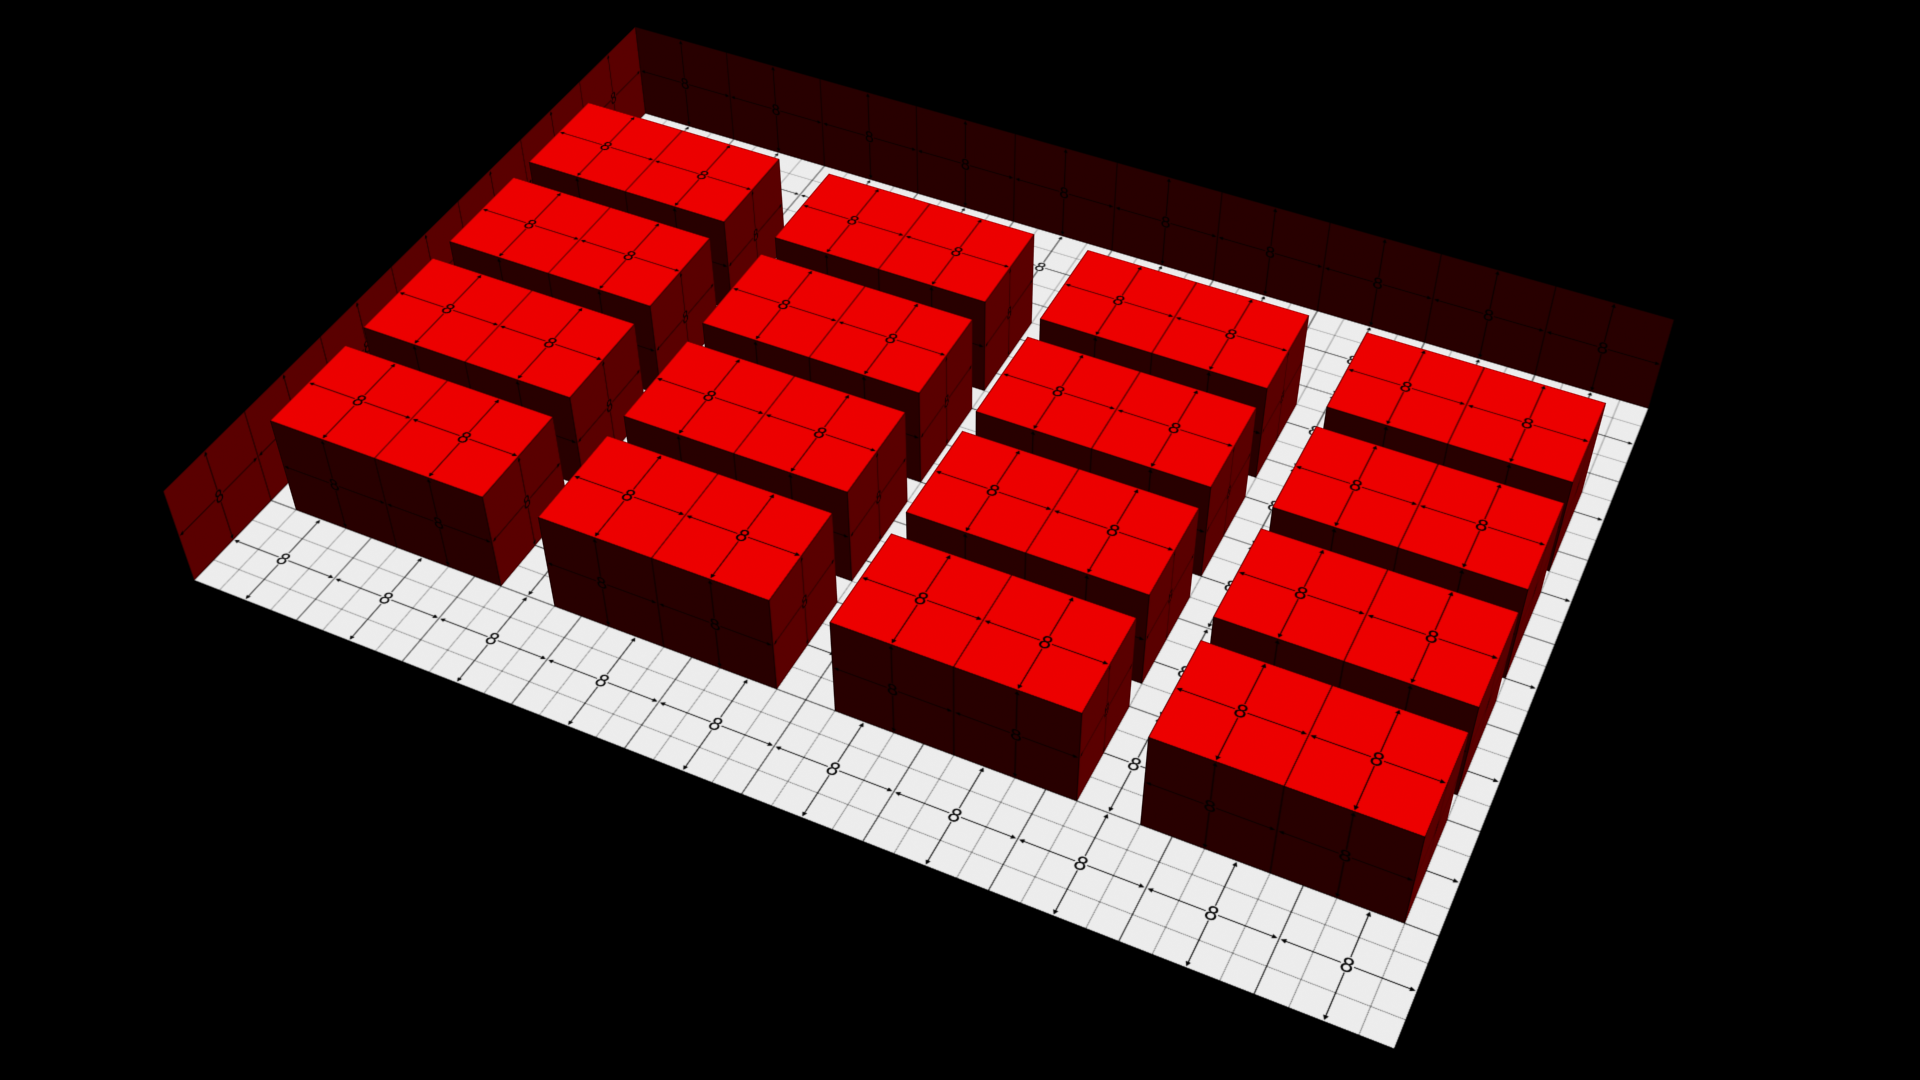
\includegraphics[scale=0.2]{frailmaprender}
    \caption{A rendering of scenery}
    \label{fig:x simmaprender}
\end{figure}

\begin{figure}[h]
    \centering
    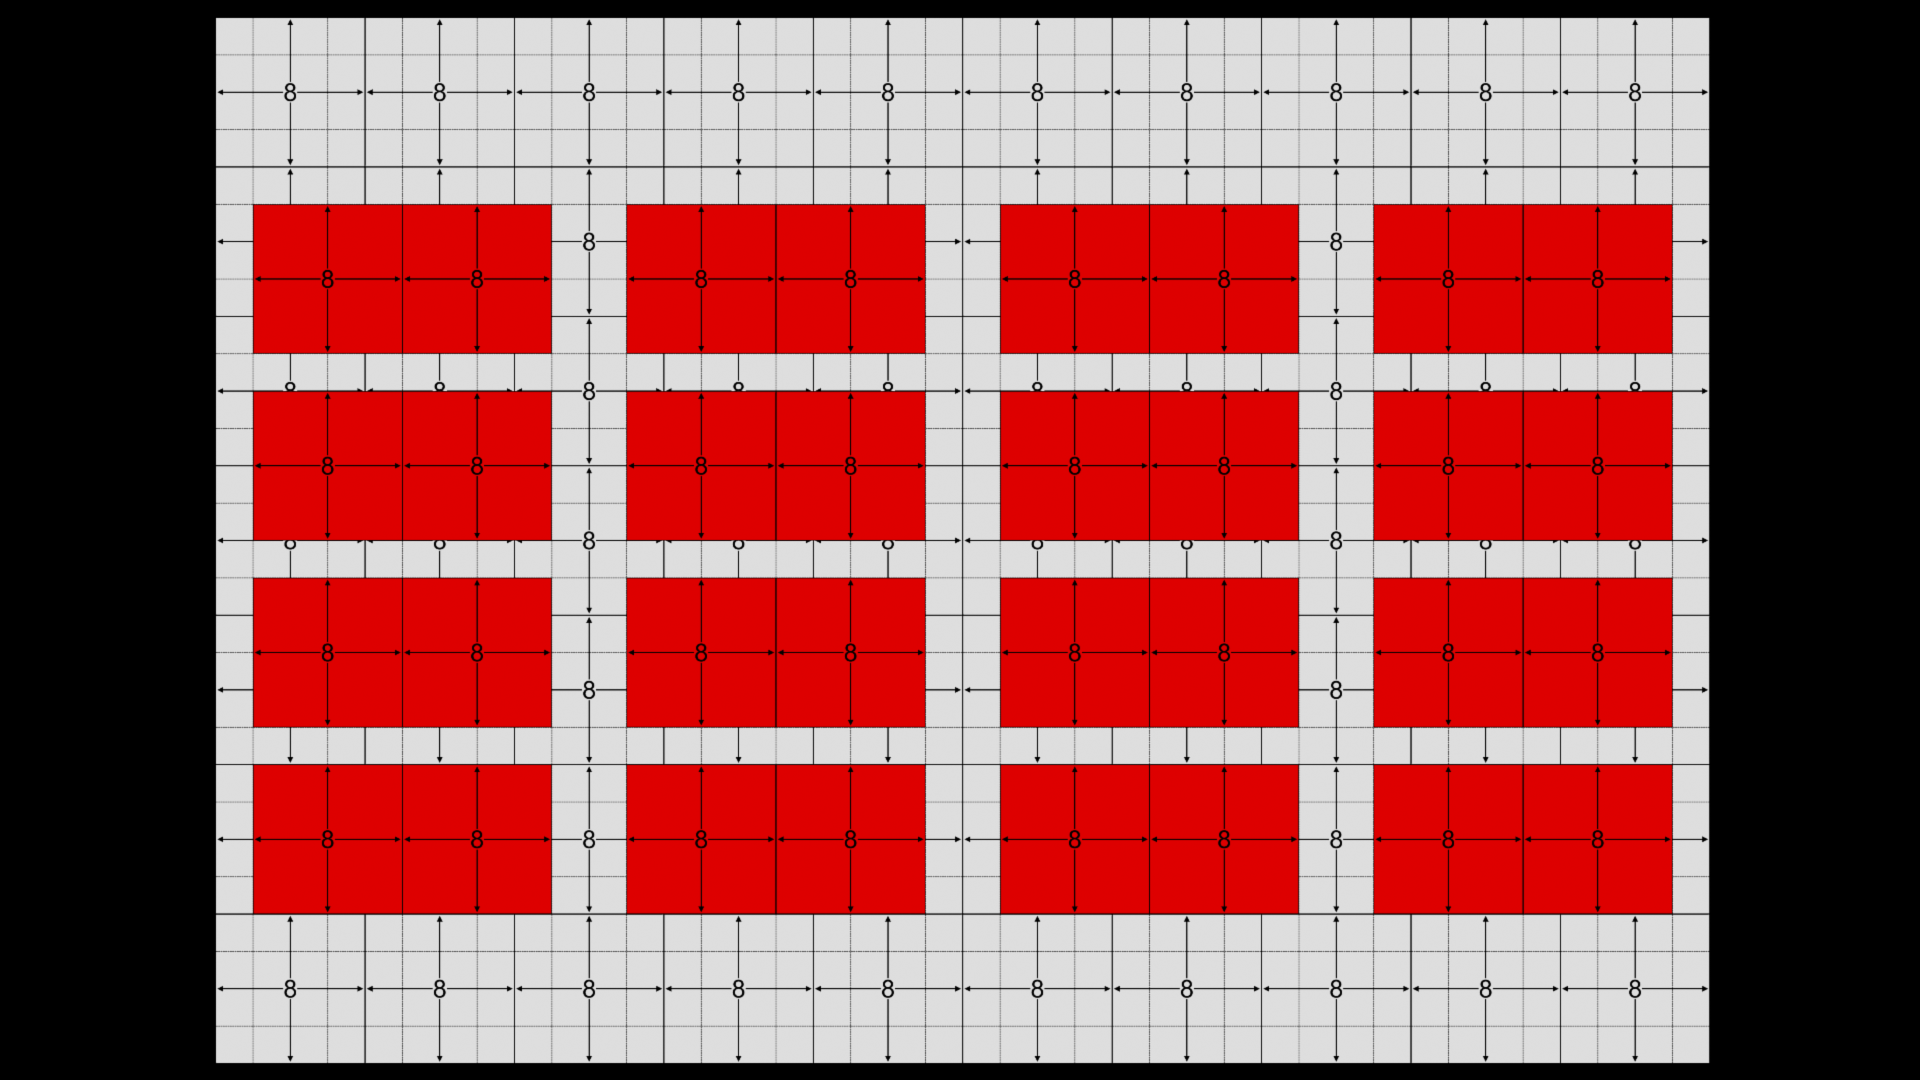
\includegraphics[scale=0.2]{frailmaptopdown}
    \caption{A top-down view of the map}
    \label{fig:x simmaptopdown}
\end{figure}

The map was designed with two to four agents in mind, with the possibility of scaling up when needed. Its shape is rectangular, measuring 80 on 56 simulation units. Over the middle secion, 14 cuboid structures were placed symmetrically to act as storage containers / shelve-holding space, with access points along every edge. This placement allowed to make use of narrow alleys between containers in order to create potential conflict points, and positioning resources right next to them would hopefully allow for more faithful representation of a real-world resource gathering problem.
